\documentclass[letterpaper,12pt]{article}

\usepackage{threeparttable}
\usepackage{geometry}
\geometry{letterpaper,tmargin=1in,bmargin=1in,lmargin=1.25in,rmargin=1.25in}
\usepackage[format=hang,font=normalsize,labelfont=bf]{caption}
\usepackage{amsmath}
\usepackage{mathrsfs}
\usepackage{multirow}
\usepackage{array}
\usepackage{delarray}
\usepackage{listings}
\usepackage{amssymb}
\usepackage{amsthm}
\usepackage{lscape}
\usepackage{natbib}
\usepackage{setspace}
\usepackage{float,color}
\usepackage[pdftex]{graphicx}
\usepackage{pdfsync}
\usepackage{verbatim}
\usepackage{placeins}
\usepackage{geometry}
\usepackage{pdflscape}
\synctex=1
\usepackage{hyperref}
\hypersetup{colorlinks,linkcolor=red,urlcolor=blue,citecolor=red}
\usepackage{bm}


\theoremstyle{definition}
\newtheorem{theorem}{Theorem}
\newtheorem{acknowledgement}[theorem]{Acknowledgement}
\newtheorem{algorithm}[theorem]{Algorithm}
\newtheorem{axiom}[theorem]{Axiom}
\newtheorem{case}[theorem]{Case}
\newtheorem{claim}[theorem]{Claim}
\newtheorem{conclusion}[theorem]{Conclusion}
\newtheorem{condition}[theorem]{Condition}
\newtheorem{conjecture}[theorem]{Conjecture}
\newtheorem{corollary}[theorem]{Corollary}
\newtheorem{criterion}[theorem]{Criterion}
\newtheorem{definition}{Definition} % Number definitions on their own
\newtheorem{derivation}{Derivation} % Number derivations on their own
\newtheorem{example}[theorem]{Example}
\newtheorem{exercise}[theorem]{Exercise}
\newtheorem{lemma}[theorem]{Lemma}
\newtheorem{notation}[theorem]{Notation}
\newtheorem{problem}[theorem]{Problem}
\newtheorem{proposition}{Proposition} % Number propositions on their own
\newtheorem{remark}[theorem]{Remark}
\newtheorem{solution}[theorem]{Solution}
\newtheorem{summary}[theorem]{Summary}
\bibliographystyle{aer}
\newcommand\ve{\varepsilon}
\renewcommand\theenumi{\roman{enumi}}
\newcommand\norm[1]{\left\lVert#1\right\rVert}

\begin{document}

\title{Econ 581 Homework 4}
\author{Chris Rytting}
\maketitle
\subsection*{Exercise 1}
Order 1 Approximation Moments

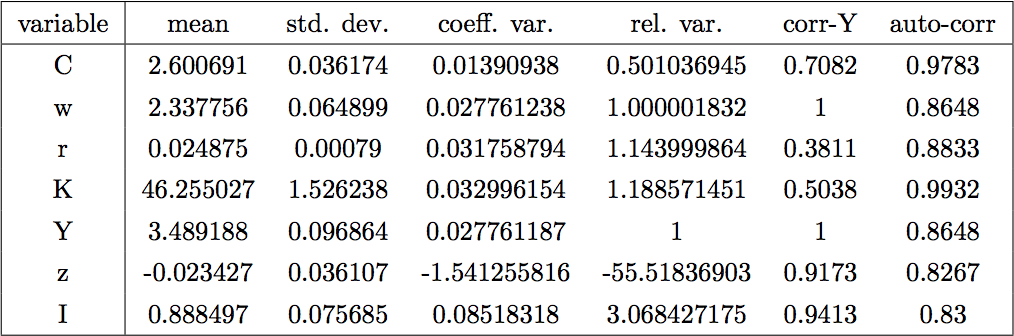
\includegraphics[scale=.75]{11.png}\\

Order 3 Approximation Moments

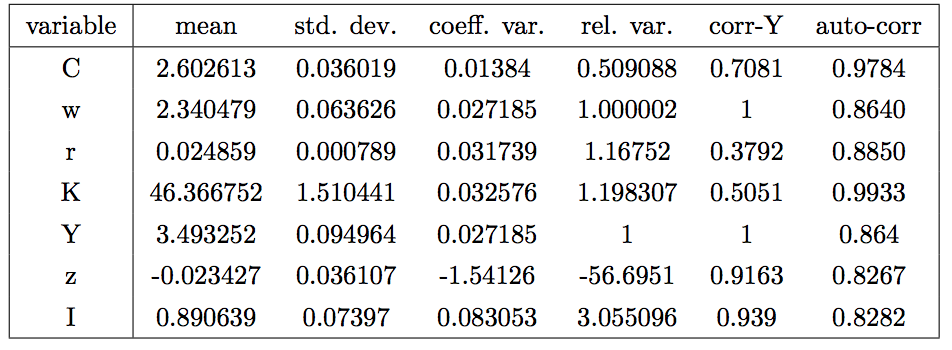
\includegraphics[scale=.75]{12.png}\\

Moments are very similar.
Our cubic approximation generates means much closer to the theoretical values. 

\subsection*{Exercise 2}
Let $\alpha = .25$.\\
Quadratic Approximation Moments

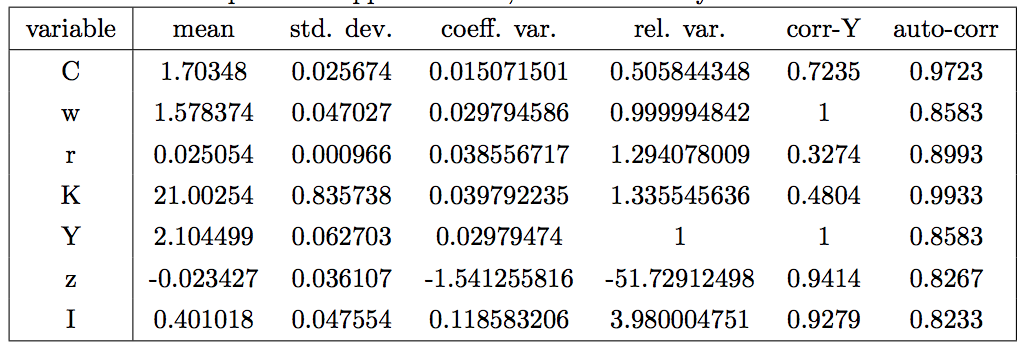
\includegraphics[trim = {0 0 0 .1cm}, clip,scale=.75]{21.png}\\

Let $\alpha = .40$.\\
Quadratic Approximation Moments

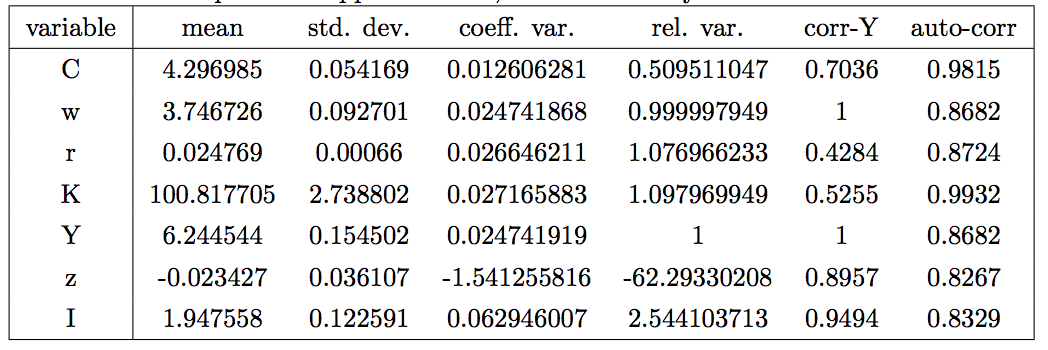
\includegraphics[trim = {0 0 0 .1cm}, clip,scale=.75]{22.png}\\

With an increase in $\alpha$, we have an increase in capital share and therefore investment. This causes an increase in GDP and consumption, but lowers the interest rate. Human capital has a higher value in the long run. The remaining moments are similar.

\subsection*{Exercise 3}
Let $\rho = 0$.\\
Quadratic Approximation Moments\\
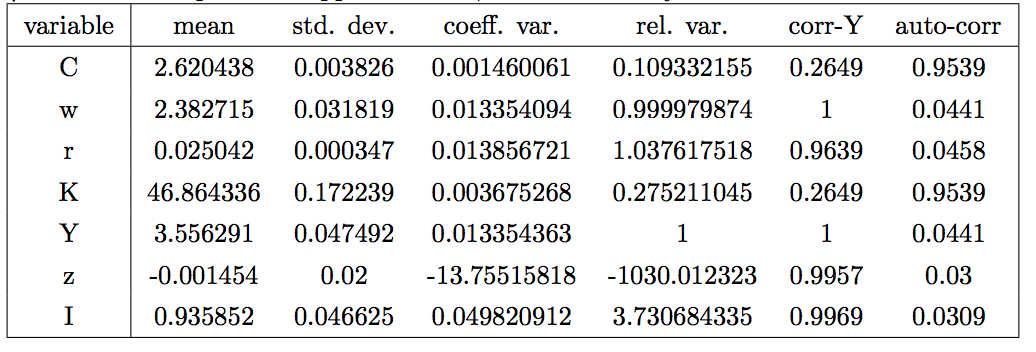
\includegraphics[trim = {0 0 0 .05cm}, clip,scale=.75]{31.png}\\


Let $\rho = 0.50$.\\
Quadratic Approximation Moments\\
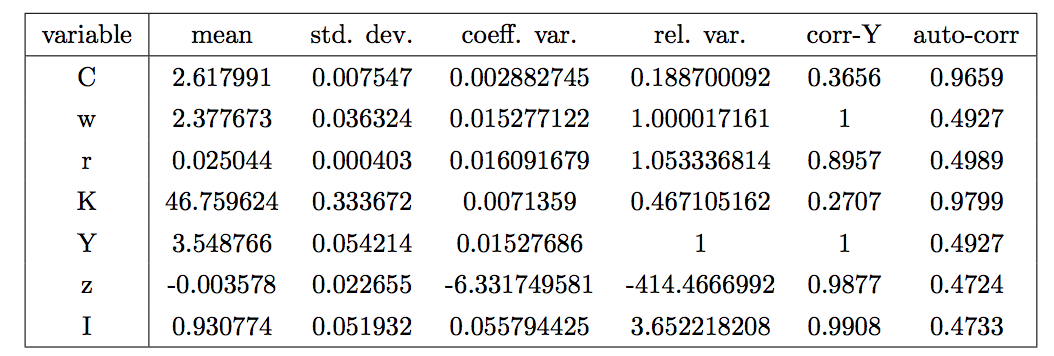
\includegraphics[scale=.75]{32.png}\\

Let $\rho = 0.99$.\\
Quadratic Approximation Moments\\
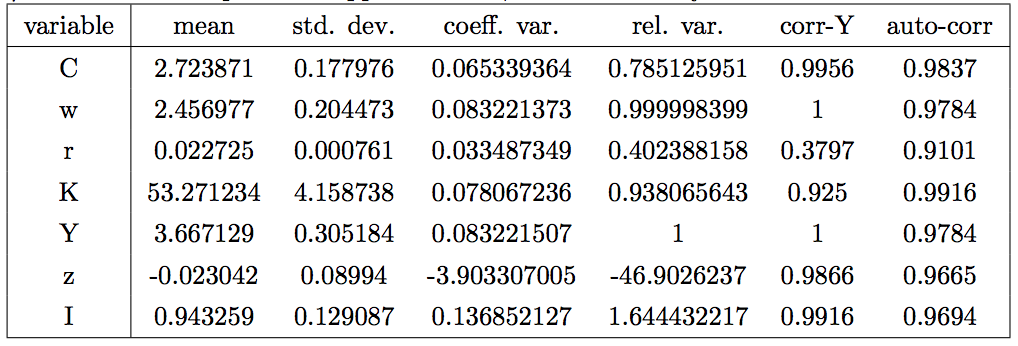
\includegraphics[trim = {0 0 0 .05cm}, clip,scale=.75]{33.png}\\

As $\rho$ increases, we have an increase in standard deviation and autocorrelation nearing 1. This happens because the residual effects of external shocks persist for longer. Interest rate not as correlated to GDP and capital stocks have a higher covariance with GDP.









\end{document}
